\documentclass{article}
\usepackage{float}
\usepackage{graphicx}
\usepackage{amsmath}
\usepackage{listings}
\usepackage{color}
\definecolor{cadmiumgreen}{rgb}{0.0, 0.42, 0.24}
\lstset{frame=tb,
  language=R,
  aboveskip=3mm,
  belowskip=3mm,
  showstringspaces=false,
  columns=flexible,
  basicstyle={\small\ttfamily},
  numbers=none,
  numberstyle=\tiny\color{gray},
  keywordstyle=\color{blue},
  commentstyle=\color{dkgreen},
  stringstyle=\color{cadmiumgreen},
  breaklines=true,
  breakatwhitespace=true,
  tabsize=3
}
\usepackage[margin=0.75in]{geometry}
\setlength\parindent{0pt}

\title{QSCI 381 HW 4}
\date{1/27/2023}
\author{Simon-Hans Edasi}

\begin{document}

	\maketitle



%%%%%%%%%%%%%%%%%%%%%%%%%%%%%%%%%%%%%%%%%%%%%%%%%%



\begin{center}
\begin{lstlisting}
data(CO2)
\end{lstlisting}
\end{center}

(1) Use R/RStudio to calculate the sample mean, sample variance, and sample standard deviation of uptake. List your answers below, rounding to two decimal places. (6 points)
\begin{center}
\begin{lstlisting}
 > mean(CO2$uptake)
[1] 27.21

> var(CO2$uptake)
[1] 116.95

> sd(CO2$uptake)
[1] 10.81
\end{lstlisting}
\end{center}



(2) Use R/RStudio to calculate the IQR of uptake. List your answer below, rounding to two decimal places (6 points)

\begin{center}
\begin{lstlisting}
 > IQR(CO2$uptake)
[1] 19.225
\end{lstlisting}
\end{center}


(3) Plot a histogram of uptake, and paste your histogram below. You can use default settings in R/RStudio for the axis labels and title. Do the data look normally distributed or not? Justify your answer. (12 points)


\begin{figure}[H]
    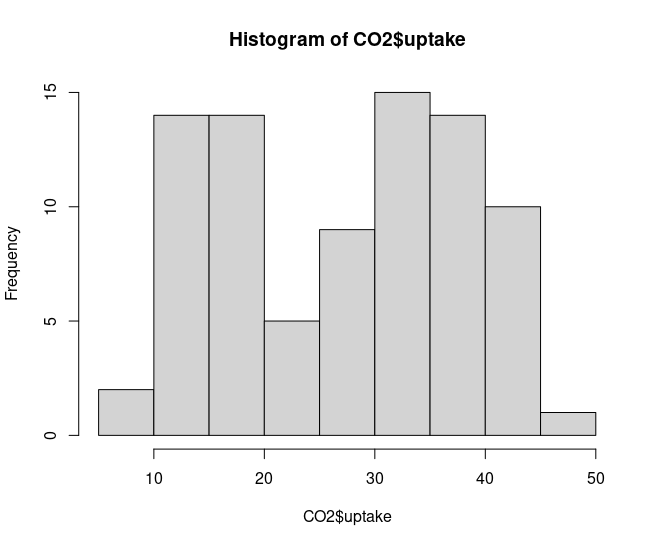
\includegraphics[scale = 0.5]{CO2_uptake_hist.png}
\end{figure}

It's hard to say, it resembles a normal distribution with some skew, but there is some massive representation in the left tail.\\

(4) In addition to the histogram, quantile-quantile plots, or Q-Q plots, are useful in assessing whether or not the data are normally distributed. In a Q-Q plot, the observed data from a sample are compared to the theoretical quantiles expected in a normal distribution. In R/RStudio, making a Q-Q plot is a two-step process: first we plot the data, and then we can add a line that represents a 1:1 relationship between the observed and theoretical quantiles. Let’s first make a Q-Q plot for the data contained in uptake. You can use default settings in R/RStudio for the axis labels and title. To do this, enter:
\begin{center}
\begin{lstlisting}
qqnorm(CO2$uptake)
\end{lstlisting}
\end{center}


With the above plot still open, overlay a 1:1 line for the Q-Q plot:

\begin{center}
\begin{lstlisting}
qqnorm(CO2$uptake)
\end{lstlisting}
\end{center}


Paste your Q-Q plot below. Based on the Q-Q plot, do the data look normally distributed or not? Justify your answer. (12 points)

\begin{figure}[H]
    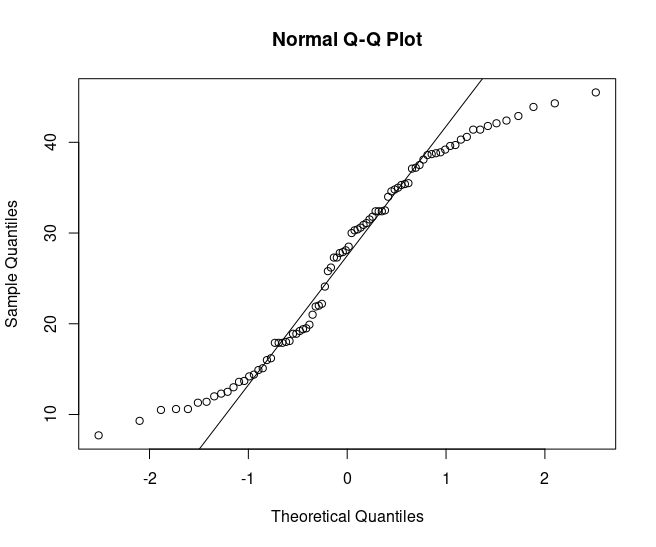
\includegraphics[scale = 0.5]{qq_normal.png}
\end{figure}

Mostly.The plot shows plot the IQRs do not follow the theoretical, but that is mostly for the edges which are strongly under-represented. The bulk of the middle of the plot does follow the theoretical though, so again it's hard to say.\\

(5) Calculate the z-score that corresponds to an uptake rate of 33.5 $\frac{\mu mol}{m^{2}s}$ and interpret the z-score relative to the mean. Be specific in your answer. (4 points)

\begin{center}
\begin{lstlisting}
> z <- (33.5 - 27.21) / 10.81
> z
[1] 0.5818686
\end{lstlisting}
\end{center}
This Z-score says that 33.5 is 0.58 standard deviation units away from the mean of 27.21, so it's a pretty typical observation.\\

In R/RStudio, we can use the following command to calculate cumulative probabilities under the normal distribution:
\begin{center}
\begin{lstlisting}
pnorm(datum, mean, sd)
\end{lstlisting}
\end{center}

which returns the cumulative probability for a specific datum, given the mean and standard deviation of the dataset.

 

Consider example 4.9 from the textbook (page 138). In this problem, we can calculate the cumulative probability of Edward's SAT score, which was 1030, given a mean SAT score of 1100 and a standard deviation of 200. To do this using pnorm():\\
\begin{center}
\begin{lstlisting}
pnorm(1030, mean = 1100, sd = 200) = 0.363
\end{lstlisting}
\end{center}


In other words, Edward's SAT score is around the 36th percentile, which means he scored better on the SAT than approximately 36\% of the students that took the SAT.\\

Use the mean and SD you calculated from question (1) and the pnorm() function in R to answer questions 6-9. For these questions, you must show your R code for full credit.\\

 

(6) The probability that an uptake rate from the sample dataset is $<15.3 \frac{\mu mol}{m^{2}s}$. Round your answer to 3 decimal places. (5 points)

\begin{center}
\begin{lstlisting}
> pnorm(15.3, mean = 27.21, sd = 10.81)
[1] 0.135
\end{lstlisting}
\end{center}

(7) The probability that an uptake rate from the sample dataset is $>42.7 \frac{\mu mol}{m^{2}s}$. Round your answer to 3 decimal places. (5 points)

\begin{center}
\begin{lstlisting}
> 1 - pnorm(42.7, mean = 27.21, sd = 10.81)
[1] 0.076
\end{lstlisting}
\end{center}

(8) The probability that an uptake rate from the sample dataset is $< 19$ or $>34 \frac{\mu mol}{m^{2}s}$. Round your answer to 3 decimal places. (5 points)\\

\begin{center}
\begin{lstlisting}
> (1 - pnorm(34, 27.21, 10.81)) + pnorm(19, 27.21, 10.81)
[1] 0.4887441
\end{lstlisting}
\end{center}


(9) The probability that an uptake rate from the sample dataset is between 21 and 29 $\frac{\mu mol}{m^{2}s}$. (5 points)

\begin{center}
\begin{lstlisting}
> 1 - pnorm(21, 27.21, 10.81) - (1 - pnorm(29, 27.21, 10.81))
[1] 0.2829336
\end{lstlisting}
\end{center}

In R/RStudio, we can use the qnorm() command to calculate a datum for a given probability:
\begin{center}
\begin{lstlisting}
qnorm(p, mean, sd)
\end{lstlisting}
\end{center}


which returns the datum that corresponds to a cumulative probability, p, given the mean and standard deviation of the dataset.\\

Reconsider Edward's SAT example where we calculated the probability of Edward's SAT score to be 0.363 given a mean SAT score of 1100 and a standard deviation of 200. If we did not know Edward's SAT score, we can use qnorm() to calculate it:
\begin{center}
\begin{lstlisting}
qnorm(0.363, mean = 1100, sd = 200) = 1029.91, or 1030
\end{lstlisting}
\end{center}


Note that the input, p, into qnorm() is a cumulative probability, much like it is for pnorm().\\

Use the mean and SD you calculated from question (1) and the qnorm() function in R to answer questions 10-12. For these questions, you must show your R code for full credit.

 

(10) Find the lowest possible uptake rate from the sample dataset that would be in the top 28th percentile. Round your answer to 2 decimal places. (5 points)
\begin{center}
\begin{lstlisting}
> qnorm(0.72, 27.21, 10.81)
[1] 33.51
\end{lstlisting}
\end{center}
 

(11) Find the highest possible uptake rate from the sample dataset that would be in the bottom 10th percentile. Round your answer to 2 decimal places. (5 points)

\begin{center}
\begin{lstlisting}
> qnorm(0.1, 27.21, 10.81)
[1] 13.36
\end{lstlisting}
\end{center}

(12) Between what values uptake rate would the middle 70\% of rates from the sample fall? Round your answer to 2 decimal places. (5 points)

\begin{center}
\begin{lstlisting}
> qnorm(0.15, 27.21, 10.81)
[1] 16.00616
> qnorm(0.85, 27.21, 10.81)
[1] 38.41384
\end{lstlisting}
\end{center}




























\end{document}
